\scanpage{172}
% archive sheet number: 171
\diagram{$\begin{array}{c|c|c|c}
\begin{smallmatrix} &F\\ V&\diagdown\end{smallmatrix}&\text{isom}&\text{épim}&\text{nilpotent}\\ \hline
\text{isom}&\text{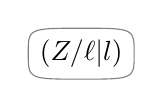
\begin{tikzpicture}[baseline=(q.base)]\node[inner sep=4pt] (q) {$(\mathbb Z/\unsure{\ell|l})$};\draw[gray,thin] (q.north) .. controls (q.north east) and (q.north east) .. (q.east) .. controls (q.south east) and (q.south east) .. (q.south) .. controls (q.south west) and (q.south west) .. (q.west) .. controls (q.north west) and (q.north west) .. cycle;\end{tikzpicture}}&\text{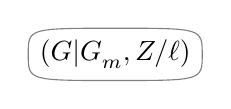
\begin{tikzpicture}[baseline=(q.base)]\node[inner sep=4pt] (q) {$({\unsure{\mathbb G|G}}_m,\mathbb Z/\ell)$};\draw[gray,thin] (q.north) .. controls (q.north east) and (q.north east) .. (q.east) .. controls (q.south east) and (q.south east) .. (q.south) .. controls (q.south west) and (q.south west) .. (q.west) .. controls (q.north west) and (q.north west) .. cycle;\end{tikzpicture}}&\text{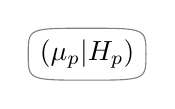
\begin{tikzpicture}[baseline=(q.base)]\node[inner sep=4pt] (q) {$(\unsure{\mu_p|H_p})$};\draw[gray,thin] (q.north) .. controls (q.north east) and (q.north east) .. (q.east) .. controls (q.south east) and (q.south east) .. (q.south) .. controls (q.south west) and (q.south west) .. (q.west) .. controls (q.north west) and (q.north west) .. cycle;\end{tikzpicture}}\\[1.2em]\hline
\begin{gathered}\deleted{\text{épim}}\\\text{mono}\end{gathered}&\begin{gathered}\text{discret \unsure{sép|si|ss}}\\ \text{\unsure{sans} }\unsure{V|p}\text{-torsion}\\(\mathbb Z/\ell,\mathbb Z)\deleted{\unsure{\mathbb Q}}\end{gathered}&\begin{gathered}\text{\unsure{multiplicatif} }\unsure{\times|+}\text{\unsure{simple|lisse}}\\\deleted{\text{\unsure{chaque groupe}}}\\\deleted{\text{\unsure{discret} }\unsure{p}\text{\unsure{-tors.}}}\\(\mathbb G_m,\mathbb Z/\ell\mathbb Z,\mathbb Z)\end{gathered}&\text{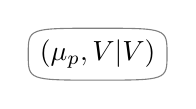
\begin{tikzpicture}[baseline=(q.base)]\node[inner sep=4pt] (q) {$(\mu_p,\unsure{\mathbb V|V})$};\draw[gray,thin] (q.north) .. controls (q.north east) and (q.north east) .. (q.east) .. controls (q.south east) and (q.south east) .. (q.south) .. controls (q.south west) and (q.south west) .. (q.west) .. controls (q.north west) and (q.north west) .. cycle;\end{tikzpicture}}\\[1.2em]\hline
\text{nilpotent}&\text{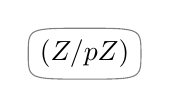
\begin{tikzpicture}[baseline=(q.base)]\node[inner sep=4pt] (q) {$(\mathbb Z/p\mathbb Z)$};\draw[gray,thin] (q.north) .. controls (q.north east) and (q.north east) .. (q.east) .. controls (q.south east) and (q.south east) .. (q.south) .. controls (q.south west) and (q.south west) .. (q.west) .. controls (q.north west) and (q.north west) .. cycle;\end{tikzpicture}}&\text{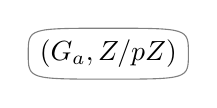
\begin{tikzpicture}[baseline=(q.base)]\node[inner sep=4pt] (q) {$(\mathbb G_a,\mathbb Z/p\mathbb Z)$};\draw[gray,thin] (q.north) .. controls (q.north east) and (q.north east) .. (q.east) .. controls (q.south east) and (q.south east) .. (q.south) .. controls (q.south west) and (q.south west) .. (q.west) .. controls (q.north west) and (q.north west) .. cycle;\end{tikzpicture}}&\begin{gathered}\deleted{\text{\unsure{groupe fini radiciel}}}\\\text{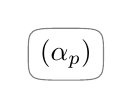
\begin{tikzpicture}[baseline=(q.base)]\node[inner sep=4pt] (q) {$(\alpha_p)$};\draw[gray,thin] (q.north) .. controls (q.north east) and (q.north east) .. (q.east) .. controls (q.south east) and (q.south east) .. (q.south) .. controls (q.south west) and (q.south west) .. (q.west) .. controls (q.north west) and (q.north west) .. cycle;\end{tikzpicture}}\end{gathered}\\\hline
\end{array}$}

Propriétés de $F,V$, \unsure{caractérisant} \unsure{l'Existence|l'existence|l'éclatement} de séries de composition ayant des propriétés données ----

\figure{
\begin{tikzpicture}[x=1cm,y=1cm]
\draw (0,0)--(6,-.06);
\draw (2,-.17)--(4.2,-.25)--(3.2,.30)--(3.25,-1.1);
\draw (4.7,-.61)--(2.3,-.50) .. controls (3.1,-.56) and (3.3,-.66) .. (3.25,-1.1);
\end{tikzpicture}}

% paper watermark: VELIN EXTRA (not author text)
